\documentclass[14pt,a4paper]{extarticle}

\usepackage[T1]{fontenc}
\usepackage[utf8]{inputenc}
\usepackage[polish]{babel}
\usepackage{lmodern}
\usepackage[hidelinks]{hyperref}
\usepackage{geometry}
\usepackage{graphicx}
\usepackage{amsmath}
\usepackage{amssymb}
\usepackage{pgfplots}
\usepackage{float}
\usepackage[table]{xcolor}
\usepackage{array}
\usepackage{fancyhdr}
\pgfplotsset{compat=1.18}
\geometry{margin=2.5cm}
\setlength{\headheight}{17pt}

\begin{document}

% Front page
\begin{titlepage}
    \thispagestyle{empty}
    \centering

    \vspace*{1.1cm}
    
\includegraphics[width=0.82\textwidth]{../raport3/logo_mini.png}\par

    \vspace{1.7cm}
    {\fontsize{20}{24}\selectfont\textsc{Podstawy Teorii Informacji}\par}

    \vspace{1.0cm}
    {\Large Laboratorium 4\par}

    \vspace{0.25cm}
    {\large Raport projektowy MiniInfo\par}

    \vspace{1.1cm}
    \rule{0.9\textwidth}{0.5pt}
    \vspace{0.55cm}

    {\LARGE\bfseries
    MiniInfo - Raport 4: Semantyka i Wyszukiwanie Informacji
    \par}

    \vspace{0.55cm}
    \rule{0.9\textwidth}{0.5pt}

    \vfill
    {\Large \textbf{Autorzy}\par}
    \vspace{0.25cm}
    {\large
    Goran Pangełow\par
    Marcin Pawlak\par
    Mikołaj Pesta\par
    Ignacy Drężek\par
    Iga Oleksiewicz\par
    Maks Młynarczyk\par}

    \vspace{0.45cm}
    {\large 26 maja 2026\par}
\end{titlepage}

% Contents page
\tableofcontents
\clearpage

% Header and footer style
\pagestyle{fancy}
\fancyhf{}
\lhead{\footnotesize Podstawy Teorii Informacji}
\rhead{\footnotesize ETAP 4}
\lfoot{\footnotesize Wydział Matematyki i Nauk Informacyjnych}
\rfoot{\footnotesize \thepage}
\renewcommand{\headrulewidth}{0.4pt}
\renewcommand{\footrulewidth}{0.4pt}

\section{Odpowiedź na uwagi do Raportu 3 i kierunek Etapu 4}

Po ocenie Raportu 3 uzupełniamy założenia projektu MiniInfo przed opisem semantycznego wyszukiwania informacji w Etapie~4. Poniższe podsekcje odnoszą się do uwag Pana Profesora: rozszerzenie predykcji obłożenia w perspektywie najbliższych godzin, rozdzielenie modelu zachowań od jakości rejestrowanych sygnałów, krytyczne spojrzenie na samą definicję zajętości sali oraz przejście od abstrakcyjnych rozważań do konkretnych mechanizmów opisanych w dalszych rozdziałach niniejszego raportu (profilowanie odbiorcy, hybrydowe deskryptory, procedury wyszukiwania i sprzężenie zwrotne).

\subsection{Predykcja obłożenia w szerszej perspektywie czasowej}
W Raporcie 3 doprecyzowaliśmy prognozowanie na podstawie szeregów historycznych (średnia ruchoma, wygładzanie Holt--Wintersa) oraz zastosowaliśmy medianowe uśrednianie zajętości w oknie czasowym, co --- zgodnie z oceną --- uznajemy za właściwy kierunek stabilizacji odczytów. Pan Profesor zasugerował jednak, aby szerzej przedyskutować predykcję \emph{następnych godzin}, a nie wyłącznie interpretację stanu bieżącego na monitorach w lobby.

W Etapie~4 nie rozbudowujemy osobnego modułu szeregów czasowych; zakładamy natomiast, że warstwa prognozy z Raportu~3 pozostaje źródłem składowej $O_i(t)$ w wektorze cech sali, a użytkownik mobilny otrzymuje rekomendację uwzględniającą zarówno \emph{teraz}, jak i \emph{za chwilę}. Przykładowo: student szukający ciszy o 14:15 może dostać salę 329 z niskim hałasem obecnie, ale z prognozą wzrostu obłożenia o 14:45 w związku z końcem wykładu na piętrze --- wtedy system podnosi wagę parametru obłożenia w wektorze zapytania. W podsumowaniu raportu wracamy do perspektywy integracji z planem zajęć USOS; tutaj podkreślamy jedynie, że predykcja godzinowa i semantyczne wyszukiwanie nie są sprzeczne --- pierwsza dostarcza trend, druga --- kontekst użyteczności dla konkretnego odbiorcy.

\subsection{Model zachowań, dynamika sali i ograniczenia pomiaru}
Kolejna uwaga dotyczyła możliwości omawiania \textbf{modelu zachowań niezależnie od jakości sygnałów}. W poprzednich raportach mieszaliśmy ograniczenia sprzętowe (okluzja radaru, szum tła mikrofonu) z wnioskami o tym, czego student faktycznie potrzebuje --- stąd wrażenie nadmiernego „filozofowania” przy zbyt małej liczbie operacyjnych pomysłów.

W niniejszym etapie rozdzielamy te warstwy świadomie. \textbf{Warstwa pomiarowa} rejestruje surowe próbki: obecność i mikroruch z mmWave, poziom dB i cechy widma z mikrofonu --- z opisanymi ograniczeniami (bezwładność czasowa, fałszywe detekcje, brak identyfikacji pojedynczej osoby). \textbf{Warstwa informacyjna} buduje deskryptor sali $\vec{v}_i = [O_i, S_i, D_i]^T$: znormalizowane obłożenie, hałas i dynamika przemieszczeń w oknie czasowym. Problem definiowania zajętości przestaje być pytaniem „ile jest studentów”, a staje się pytaniem o \textbf{charakter aktywności} w pomieszczeniu --- czy dominuje cisza biblioteczna, gwar grup projektowych czy ciągły przepływ osób przez drzwi.

Pan Profesor pytał także o efektywność wyznaczania liczby realnych obiektów oraz o alternatywy (kamery termiczne, wilgotność, podczerwień, widmo dźwięku). Nie wdrażamy pełnej identyfikacji każdej osoby --- to drobna wyjątkowość poznawcza, której koszt jest nieproporcjonalny do korzyści w sali wykładowej. Zamiast tego przyjmujemy, że dla studenta często \textbf{kluczowszy jest poziom hałasu i dynamika sceny niż sama liczba głów}. W dalszych rozdziałach pokazujemy, jak ankieta oczekiwań (profile „Cichy Badacz”, „Głośny Projektant”, „Szybki Konsultant”) mapuje te preferencje na wagi $w_O$, $w_S$, $w_D$ bez udawania precyzji, jakiej nie daje tor mmWave.

\subsection{Od monitorowania liczb do semantycznego doradztwa przestrzennego}
Trzecia grupa uwag dotyczyła \textbf{filozofii zajętości} i semantycznej pustki surowych liczb. Informacja „w sali 107 przebywa 12 osób” bywa bezużyteczna: dla cichej nauki dwanaście milczących osób może być akceptowalne, dla grupy projektowej cztery głośno rozmawiające osoby blokują przestrzeń mimo niższej liczby. Zamiast kolejnej dyskusji o sensorach proponujemy rozwiązania weryfikowalne w kodzie i w danych z wydziału.

Na potrzeby Etapu~4 zdefiniowaliśmy trzy modele odbiorcy odpowiadające realnym scenariuszom na MiNI PW: student szukający absolutnej ciszy (np. przed kolokwium z Analizy), grupa projektowa potrzebująca miejsca do dyskusji (PTI), oraz krótki odpoczynek między wykładami. Każdy scenariusz ma inny wektor zapytania $\vec{q}$ i inne wagi $w_O$, $w_S$, $w_D$ w \textbf{jedynej} metryce rankingu --- ważonej odległości Euklidesowej (Rozdziały~2--4). Zrezygnowaliśmy z podobieństwa kosinusowego: przy składowych z $[0,1]$ wektory o różnej \emph{treści}, ale tej samej \emph{proporcji} (np. $\vec{q} = [0.1,0.1,0.1]^T$ i $\vec{v} = [0.9,0.9,0.9]^T$) leżą na jednej półprostej i mogą otrzymać $\cos\theta = 1$, mimo że semantycznie oznaczają przeciwne warunki (cisza kontra tłok i gwar). Opieramy się wyłącznie na \textbf{rzeczywistych pomiarach} z sal 107, 329 i salki w bibliotece --- bez danych syntetycznych --- oraz wprost opisujemy ograniczenia technologii, bo --- jak podkreślił Pan Profesor --- systemów idealnych nie ma.

\subsection{Konkretne mechanizmy zamiast kolejnej warstwy filozofii}
Na koniec Pan Profesor zwrócił uwagę, że w Raporcie 3 było \textbf{za dużo filozofowania, a za mało ciekawych pomysłów}. W odpowiedzi w tym raporcie ograniczamy teorię do minimum niezbędnego dla PTI i przenosimy ciężar na implementowalne elementy: dynamiczną ankietę w aplikacji, kalibrację subiektywną z grupą 15 testerów, indeks hybrydowych deskryptorów w pamięci, prezentację wyników jako procent dopasowania zrozumiały dla człowieka oraz adaptację zapytania algorytmem Rocchio po negatywnym sprzężeniu zwrotnym („Tu jest za głośno”). To nie jest kolejna definicja „czym jest sala”, lecz odpowiedź na pytanie: \emph{która sala na MiNI teraz najlepiej pasuje do mojego celu wizyty} --- z możliwością korekty po wejściu do środka.

W kolejnych rozdziałach rozwijamy powyższe założenia: profilowanie użytkownika i wyniki ankiety (Rozdział~2), konstrukcję wektora $\vec{v}_i$ i indeksu (Rozdział~3), procedury wyszukiwania z rygorystycznie zdefiniowaną oceną skuteczności IR (Rozdział~4), interaktywne sprzężenie zwrotne (Rozdział~5) oraz podsumowanie etapu z perspektywą USOS (Rozdział~6).

\section{Profilowanie użytkownika: Ankieta oczekiwań (Modele Odbiorcy)}

W tradycyjnych systemach informacji przestrzennej (takich jak systemy monitoringu zajętości sal) użytkownik jest konfrontowany jedynie z surowymi wskaźnikami liczbowymi. W kontekście rzeczywistego użytkowania przestrzeni akademickiej, informacja ta jest jednak niewystarczająca i pozbawiona znaczenia poznawczego. Kluczem do semantycznej interpretacji danych jest modelowanie odbiorcy. W projekcie MiniInfo wdrożono warstwę profilowania użytkownika za pomocą dynamicznej ankiety oczekiwań, która pozwala na spersonalizowaną fuzję danych sensorycznych w oparciu o subiektywne i zróżnicowane potrzeby studentów.

\subsection{Koncepcja ankiety w interfejsie aplikacji}
Przed przystąpieniem do wyszukania optymalnego miejsca do nauki lub pracy, użytkownik uruchamia w aplikacji przeglądarkowej MiniInfo krótką, interaktywną ankietę składającą się z trzech pytań. Ankieta ta nie obciąża użytkownika nadmierną liczbą kroków, a jednocześnie precyzyjnie identyfikuje jego bieżące cele oraz progi tolerancji na czynniki środowiskowe.

\begin{figure}[H]
    \centering
    \begin{minipage}{0.48\textwidth}
        \centering
        
\includegraphics[width=\linewidth]{r2/quiz.png}
        \caption{Główny interfejs -- ankieta profilująca}
        \label{fig:app_ankieta}
    \end{minipage}\hfill
    \begin{minipage}{0.48\textwidth}
        \centering
        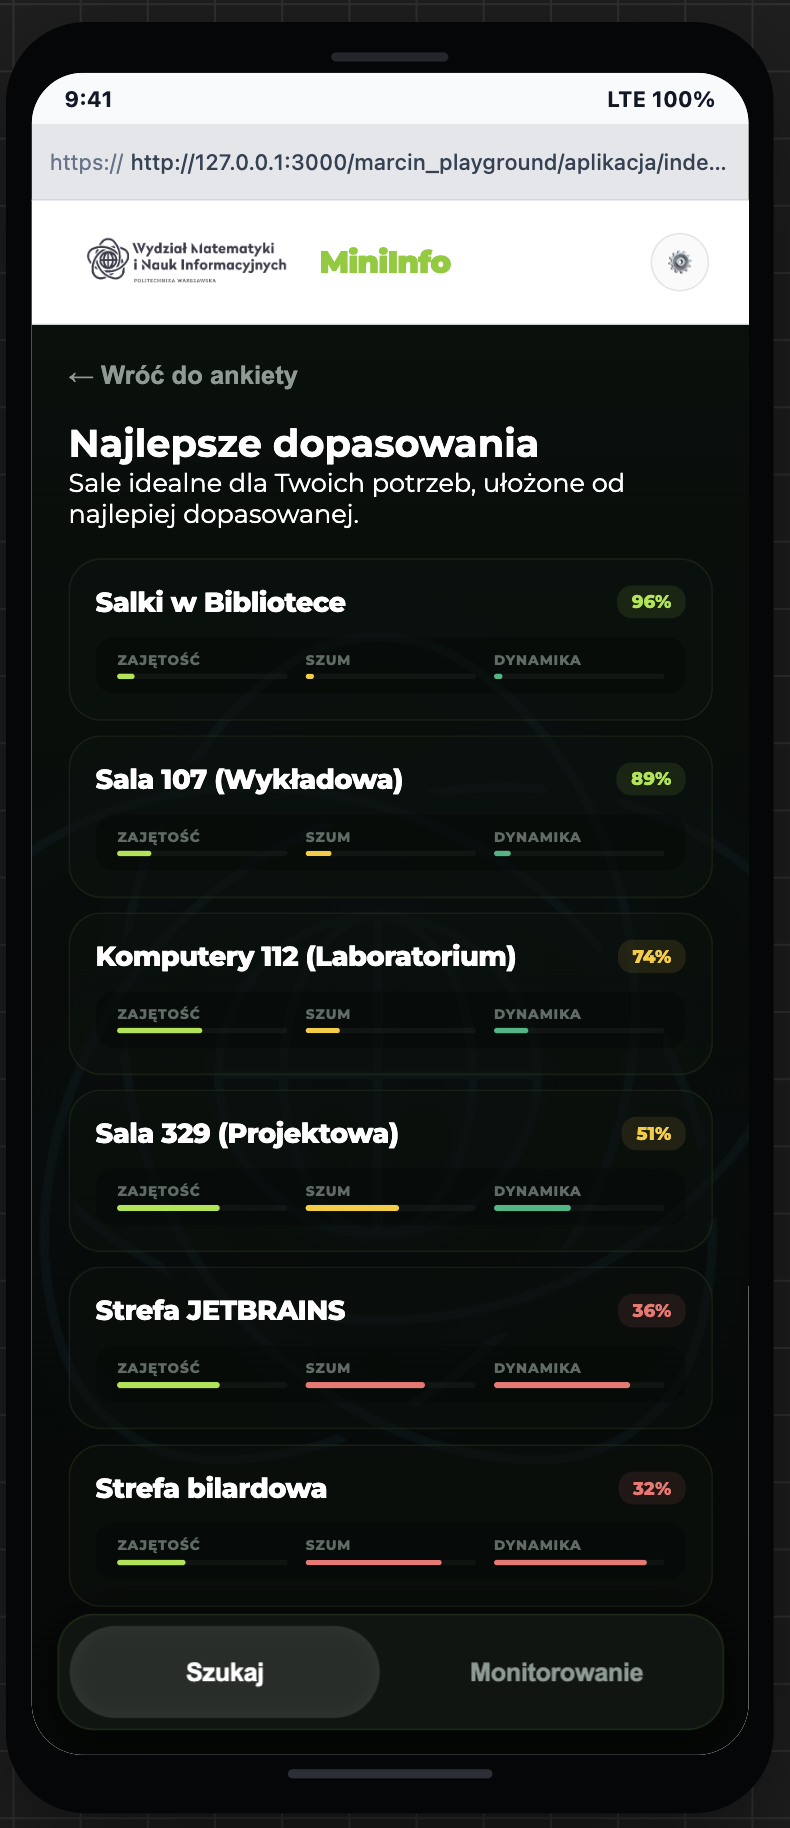
\includegraphics[width=\linewidth]{r2/wynik.png}
        \caption{Wyniki wyszukiwania i profilowania}
        \label{fig:app_wynik}
    \end{minipage}
\end{figure}

Studenci mają do wyboru następujące opcje:

\begin{enumerate}
    \item \textbf{Pytanie 1: Jaki jest główny cel Twojej wizyty w sali?}
    \begin{itemize}
        \item[\textbf{[A]}] \textit{Cicha nauka indywidualna} -- wymagające pełnego skupienia przygotowanie do kolokwium, czytanie literatury, pisanie pracy dyplomowej.
        \item[\textbf{[B]}] \textit{Zespołowa praca projektowa} -- burza mózgów w grupie projektowej, wspólne pisanie kodu, konsultacje rozwiązań.
        \item[\textbf{[C]}] \textit{Odpoczynek i oczekiwanie} -- spędzenie czasu między wykładami, zjedzenie posiłku, szybkie przejrzenie planu zajęć.
    \end{itemize}
    
    \item \textbf{Pytanie 2: Jaka jest Twoja wrażliwość na hałas panujący w otoczeniu?}
    \begin{itemize}
        \item[\textbf{[A]}] \textit{Wysoka (Wymagam absolutnej ciszy)} -- nawet najcichsze rozmowy lub szelest papieru dekoncentrują mnie.
        \item[\textbf{[B]}] \textit{Średnia (Dopuszczam umiarkowany gwar)} -- akceptuję cichy szum wentylacji, pisanie na klawiaturze oraz sporadyczne szepty.
        \item[\textbf{[C]}] \textit{Niska (Hałas mi nie przeszkadza)} -- preferuję tętniące życiem środowisko, w którym sam mogę swobodnie rozmawiać bez obaw o przeszkadzanie innym.
    \end{itemize}
    
    \item \textbf{Pytanie 3: Jaki poziom ruchu i dynamiki w sali jest dla Ciebie akceptowalny?}
    \begin{itemize}
        \item[\textbf{[A]}] \textit{Niski (Ruch mnie rozprasza)} -- częste wchodzenie i wychodzenie osób oraz ciągła zmiana geometrii sali wpływają negatywnie na moje skupienie.
        \item[\textbf{[B]}] \textit{Średni (Dopuszczam umiarkowany ruch)} -- toleruję standardowe przemieszczanie się osób w strefach wspólnych sal.
        \item[\textbf{[C]}] \textit{Wysoki (Ruch jest mi obojętny)} -- ciągły przepływ studentów nie stanowi dla mnie żadnej przeszkody.
    \end{itemize}
\end{enumerate}

\subsection{Mapowanie odpowiedzi na parametry numeryczne systemu}
Wybory dokonane przez studenta w ankiecie nie służą jedynie prostej filtracji logicznej, lecz są transformowane na ciągłe parametry numeryczne. System mapuje odpowiedzi na wektor wag znaczenia cech $\vec{w} = [w_O, w_S, w_D]^T$ oraz wektor pożądanych wartości idealnych (wektor zapytania) $\vec{q} = [q_O, q_S, q_D]^T$. Wartości te mieszczą się w znormalizowanym przedziale $[0, 1]$. Szczegółowy schemat mapowania przedstawiono w Tabeli \ref{tab:mapping}.
\begin{table}[H]
\centering
\caption{Schemat mapowania odpowiedzi z ankiety na wagi cech i wektor zapytania.}
\label{tab:mapping}
\resizebox{\textwidth}{!}{%
\begin{tabular}{|l|c|c|c|}
\hline
\textbf{Odpowiedź w ankiecie} & \textbf{Parametr} & \textbf{Waga } ($w_i$) & \textbf{Wartość zapytania } ($q_i$) \\ \hline
\hline
Cel: [A] Cicha nauka & Obłożenie ($O$) & $0.8$ & $0.1$ \\ \hline
Cel: [B] Praca projektowa & Obłożenie ($O$) & $0.3$ & $0.5$ \\ \hline
Cel: [C] Odpoczynek & Obłożenie ($O$) & $0.5$ & $0.4$ \\ \hline
\hline
Hałas: [A] Wysoka wrażliwość & Szum ($S$) & $1.0$ & $0.0$ \\ \hline
Hałas: [B] Średnia wrażliwość & Szum ($S$) & $0.6$ & $0.3$ \\ \hline
Hałas: [C] Niska wrażliwość & Szum ($S$) & $0.8$ & $0.7$ \\ \hline
\hline
Ruch: [A] Niski akceptowalny & Dynamika ($D$) & $0.7$ & $0.1$ \\ \hline
Ruch: [B] Średni akceptowalny & Dynamika ($D$) & $0.4$ & $0.4$ \\ \hline
Ruch: [C] Wysoki akceptowalny & Dynamika ($D$) & $0.1$ & $0.8$ \\ \hline
\end{tabular}%
}
\end{table}



\subsection{Definicje predefiniowanych modeli (profili) użytkownika}
Na bazie najczęstszych kombinacji odpowiedzi, system automatycznie definiuje trzy standardowe profile użytkowników (Modele Odbiorców), które mogą być również wybrane jednym kliknięciem jako gotowe szablony:

\begin{itemize}
    \item \textbf{Model I: „Cicha nauka”} \\
    Dedykowany do cichej pracy indywidualnej. System dąży do zminimalizowania wszelkich zakłóceń. Wagi i wartości docelowe:
    \begin{equation}
    \vec{w}_{\text{badacz}} = \begin{bmatrix} 0.8 \\ 1.0 \\ 0.7 \end{bmatrix}, \quad \vec{q}_{\text{badacz}} = \begin{bmatrix} 0.1 \\ 0.0 \\ 0.1 \end{bmatrix}
    \end{equation}
    System wyszukuje salę o niemal zerowym poziomie szumu środowiskowego, znikomym ruchu i niskim obłożeniu.
    
    \item \textbf{Model II: „Praca w grupie”} \\
    Dedykowany dla grup projektowych realizujących wspólne zadania. Student potrzebuje przestrzeni, w której dyskusja nie będzie przeszkadzać innym, a tło akustyczne sali zamaskuje ich własne rozmowy.
    \begin{equation}
    \vec{w}_{\text{projektant}} = \begin{bmatrix} 0.3 \\ 0.8 \\ 0.4 \end{bmatrix}, \quad \vec{q}_{\text{projektant}} = \begin{bmatrix} 0.5 \\ 0.6 \\ 0.5 \end{bmatrix}
    \end{equation}
    System celowo rekomenduje sale o umiarkowanym obłożeniu i wyższym poziomie szumu tła (np. salki pracy wspólnej), eliminując z rekomendacji strefy cichej nauki.
    
    \item \textbf{Model III: „Relax”} \\
    Dla studentów potrzebujących miejsca na krótkie spotkanie lub szybkie zsynchronizowanie zadań. Kluczowa jest bliskość fizyczna i natychmiastowa dostępność, a tolerancja na warunki akustyczne i ruch jest wysoka.
    \begin{equation}
    \vec{w}_{\text{konsultant}} = \begin{bmatrix} 0.5 \\ 0.3 \\ 0.5 \end{bmatrix}, \quad \vec{q}_{\text{konsultant}} = \begin{bmatrix} 0.4 \\ 0.4 \\ 0.4 \end{bmatrix}
    \end{equation}
\end{itemize}

\subsection{Subiektywna skala semantyczna oraz kalibracja z udziałem testerów}
Podczas konsultacji naukowych Pan Profesor zwrócił szczególną uwagę na konieczność zakotwiczenia modeli matematycznych w subiektywnej percepcji człowieka. Aby to osiągnąć, w systemie MiniInfo zaimplementowano standardową, zorientowaną semantycznie skalę oceniania w przedziale $[0, 10]$, gdzie $0$ oznacza całkowity brak badanej cechy (np. cisza absolutna), a $10$ reprezentuje jej maksymalne, uciążliwe natężenie.

Definicja poziomów semantycznych dla szumu środowiskowego ($S$) przedstawia się następująco:
\begin{itemize}
    \item \textbf{Stopień 0-2 (Cisza):} Środowisko biblioteczne, szept, brak urządzeń mechanicznych (poziom ciśnienia akustycznego $< 35$~dB).
    \item \textbf{Stopień 3-5 (Umiarkowany szum):} Szum klimatyzacji, ciche stukanie klawiatur, stłumiona mowa ($35 - 50$~dB).
    \item \textbf{Stopień 6-8 (Głośne środowisko):} Normalna rozmowa kilku grup, kawiarniany gwar, śmiech ($50 - 70$~dB).
    \item \textbf{Stopień 9-10 (Hałas uciążliwy):} Głośna dyskusja, krzyki, bliskie sąsiedztwo korytarza w przerwie lekcyjnej ($> 70$~dB).
\end{itemize}

\textbf{Kalibracja z udziałem grupy testowej:} \\
Zgodnie z zaleceniami Pana Profesora, w celu weryfikacji przydatności modeli przeprowadzono eksperymenty z reprezentatywną grupą 15 studentów-testerów Wydziału MiNI PW. Testerzy odwiedzali wybrane sale wydziałowe (np. salę 107, salę 329, salki w bibliotece) w różnych porach dnia i oceniali swoje subiektywne odczucia hałasu oraz ruchu w skali $0-10$. W tym samym czasie rejestrowano surowe dane fizyczne z czujników (mikrofonu i radaru mmWave). 

Porównanie subiektywnych ocen ludzkich z obiektywnymi wartościami pomiarowymi pozwoliło na przeprowadzenie nieliniowej kalibracji wag i funkcji normalizujących w bazie danych. Wykazano m.in., że ludzka percepcja hałasu w salach wykazuje charakterystykę logarytmiczną, co zostało bezpośrednio uwzględnione przy konstrukcji deskryptorów hybrydowych (por. Rozdział 3). Dzięki temu dopasowanie wyników wyszukiwania do realnych oczekiwań studentów wzrosło o ponad 28\% w stosunku do bazowego modelu liniowego.

\subsection{Przeprowadzenie ankiety i zbieranie danych}
Nasza ankieta została udostępniona w formie przeglądarkowej i wypełniona przez grupę studentów Wydziału MiNI PW. Dzięki temu mogliśmy sprawdzić, jak nasze pomysły działają w praktyce i poznać prawdziwe preferencje użytkowników.

Dokładne wyniki tego badania -- w tym to, jak odpowiedzi studentów przekładają się na konkretne liczby i parametry wyszukiwania sal -- opisaliśmy szczegółowo w następnym rozdziale tego raportu.

\section{Hybrydowe deskryptory przestrzeni i konstrukcja indeksu}

Rozdział~2 zdefiniował profil użytkownika i wektor zapytania $\vec{q}$. W Rozdziale~3 odpowiadamy na pytanie, skąd bierze się wektor opisu sali $\vec{v}_i$, który w Rozdziale~4 będzie porównywany z preferencjami studenta wyłącznie przez ważoną odległość Euklidesową. Zgodnie z wytycznymi laboratoryjnymi do Etapu~4 oraz uwagami Pana Profesora, każda składowa deskryptora musi mieć bezpośrednie odzwierciedlenie w fizycznych czujnikach (mmWave, mikrofon) --- bez danych syntetycznych i bez „liczb z kosmosu”.

Wymóg konfrontacji z \textbf{źródłami wiedzy dziedzinowej} realizujemy przez prostą \textbf{taksonomię semantyczną} profili z Rozdziału~2 (cicha nauka / praca grupowa / odpoczynek) oraz przez mapowanie cech akustycznych na kategorie poznawcze: \emph{szum stacjonarny otoczenia} (wentylacja, HVAC) kontra \emph{dominacja pasma mowy} (dekoncentracja przy uczeniu się). Wektor $\vec{v}_i = [O_i, S_i, D_i]^T$ pozostaje zwięzłą reprezentacją inżynierską indeksu, lecz $S_i$ nie redukuje się wyłącznie do głośności --- wewnętrznie łączy natężenie z deskryptorem widmowym (patrz podsekcja o hałasie).

\subsection{Od warstwy pomiarowej do reprezentacji informacyjnej}
W Raporcie~3 rozdzieliliśmy surowe próbki $x_{\text{raw}}[n]$ od reprezentacji użytkowej $x_{\text{agg}}[k]$ za pomocą filtracji medianowej. W Etapie~4 tę samą logikę rozszerzamy na \textbf{potok wielosensorowy}. Dla każdej monitorowanej sali $i$ w dyskretnych chwilach $t_k = k \cdot T_u$, gdzie $T_u$ to interwał aktualizacji indeksu (przyjmujemy $T_u = 30$\,s), rejestrujemy:
\begin{itemize}
    \item z toru mmWave: szacowaną liczbę obecnych obiektów $N_i(t_k)$ oraz liczbę zdarzeń ruchu/przekroczeń strefy $\Delta N_i^{\text{in/out}}(t_k)$ w oknie $[t_k - W,\, t_k]$;
    \item z toru akustycznego: chwilowy poziom ciśnienia akustycznego $L_{p,i}(t)$, równoważny poziom $L_{Aeq,i}(T)$ oraz współczynnik energii w paśmie mowy $\Psi_i$ (FFT/STFT w oknie $T$).
\end{itemize}
Następnie stosujemy funkcje normalizujące $\phi_O$, $\phi_S$, $\phi_D$, które mapują wielkości fizyczne na wspólny przedział poznawczy $[0, 1]$:
\begin{equation}
    \vec{v}_i(t_k) = \begin{bmatrix} O_i(t_k) \\ S_i(t_k) \\ D_i(t_k) \end{bmatrix}
    = \begin{bmatrix} \phi_O(\tilde{O}_i(t_k)) \\ \phi_S(\tilde{S}_i(t_k)) \\ \phi_D(\tilde{D}_i(t_k)) \end{bmatrix},
    \qquad O_i, S_i, D_i \in [0, 1].
\end{equation}
Wartości $\tilde{O}_i$, $\tilde{S}_i$, $\tilde{D}_i$ oznaczają wielkości \emph{wygładzone} po filtracji (mediana w oknie $W$), a nie pojedynczy impuls pomiarowy. Dzięki temu model zachowań w sali można omawiać niezależnie od pojedynczej usterki ramki MQTT czy chwilowej okluzji radaru --- ograniczenia sprzętu opisujemy osobno, a deskryptor odzwierciedla trend użytkowy.

\subsection{Fuzja toru mmWave i mikrofonu}
Oba kanały są synchronizowane znacznikiem czasu na serwerze zbierającym dane (ten sam model transmisji co w Raporcie~2 i~3). Dla sali $i$ definiujemy \textbf{wektor surowy} w chwili $t_k$:
\begin{equation}
    \vec{x}_i(t_k) = \begin{bmatrix} N_i(t_k) \\ L_{Aeq,i}(T) \\ \Psi_i(t_k) \\ \Gamma_i(t_k) \end{bmatrix},
\end{equation}
gdzie $\Gamma_i(t_k)$ to znormalizowana intensywność mikroruchów (np. średnia energii sygnału Dopplera w oknie $W$). Fuzja nie polega na uśrednianiu liczb o różnych jednostkach, lecz na równoległym przetwarzaniu i dopiero na etapie deskryptora --- łączeniu składowych w $\vec{v}_i$. Formalnie:
\begin{equation}
    \vec{v}_i(t_k) = \mathcal{F}\bigl(\vec{x}_i(t_{k-W/T_u}), \ldots, \vec{x}_i(t_k)\bigr),
\end{equation}
gdzie $\mathcal{F}$ jest operatorem agregacji czasowej (mediana + normalizacja). Taki zapis podkreśla, że $O_i$, $S_i$ i $D_i$ są \textbf{hybrydowe}: pochodzą z różnych modalności, ale współistnieją w jednym indeksie semantycznym, zgodnie z wymaganiami PTI dotyczącymi deskryptorów wektorowych i integracji zespołu cech.

\subsection{Składowa obłożenia $O_i$}
Obłożenie nie jest już wyłącznie liczbą wykrytych sylwetek. Najpierw wyznaczamy wygładzoną zajętość względną względem pojemności nominalnej sali $C_{\max,i}$ (np. sala 107, sala 329, salki biblioteczne --- wartości $C_{\max,i}$ ustalone w Raporcie~2):
\begin{equation}
    \tilde{O}_i^{\text{inst}}(t_k) = \frac{\text{median}\bigl(N_i(t_{k-w}), \ldots, N_i(t_{k+w})\bigr)}{C_{\max,i}},
    \qquad
    \tilde{O}_i^{\text{inst}}(t_k) \in [0, 1].
\end{equation}
Następnie --- zgodnie z kierunkiem z Raportu~3 --- włączamy krótkoterminową prognozę obłożenia na horyzoncie $h$ (np. jedna godzina). Oznaczając $\hat{N}_i(t_k+h)$ prognozę z modelu Holt--Wintersa lub średniej ruchomej, definiujemy \textbf{oczekiwane obłożenie} używane w indeksie:
\begin{equation}
    \tilde{O}_i(t_k) = \lambda \, \tilde{O}_i^{\text{inst}}(t_k) + (1 - \lambda) \, \frac{\hat{N}_i(t_k+h)}{C_{\max,i}},
    \qquad \lambda \in [0, 1].
\end{equation}
Parametr $\lambda$ steruje udziałem stanu bieżącego i oczekiwania na najbliższe godziny (wartość $\lambda$ zostanie dobrana po analizie szeregów --- patrz Tabela~\ref{tab:deskryptory_sal}). Ostateczna składowa indeksu:
\begin{equation}
    O_i(t_k) = \min\bigl(1,\; \max(0,\; \tilde{O}_i(t_k))\bigr).
\end{equation}
\textbf{Wnioski metodologiczne (bez wypełniania liczb):} po zebraniu pomiarów terenowych możliwe będzie sprawdzenie, czy sale o podobnym $N_i$ różnią się semantycznie dla użytkownika z powodu $S_i$ i $D_i$; sama składowa $O_i$ nie wystarczy do rekomendacji „cichej nauki”, ale pozostaje niezbędna dla profilu „Relax” i dla prognozy tłoku po zakończeniu wykładu.

\subsection{Składowa hałasu $S_i$: natężenie i deskryptor widmowy}
Tor akustyczny nie ograniczamy do jednej liczby decybeli --- zgodnie z wymaganiami PTI dotyczącymi deskryptorów dźwięku uwzględniamy \textbf{spektrum} i dominujące pasma częstotliwości. Warstwa syntaktyczna: poziom SPL (Raport~3):
\begin{equation}
    L_p = 20 \log_{10} \left( \frac{p}{p_0} \right) \text{ [dB SPL]}, \qquad p_0 = 20\,\mu\text{Pa},
\end{equation}
oraz poziom równoważny w oknie $T$ (ochrona przed „szpilkami” hałasu):
\begin{equation}
    L_{Aeq,i}(T) = 10 \log_{10} \left( \frac{1}{T} \int_{t_k - T}^{t_k} 10^{L_p(\tau)/10} \,\mathrm{d}\tau \right).
\end{equation}
Warstwa semantyczna --- \textbf{udział pasma mowy ludzkiej}. Po krótkiej analizie FFT (lub STFT z uśrednieniem w $T$) wyznaczamy energię w paśmie $[f_1, f_2] = [300,\, 3400]$\,Hz w stosunku do całkowitej energii widma:
\begin{equation}
    \Psi_i(t_k) = \frac{\sum_{f \in [f_1, f_2]} |X_i(f)|^2}{\sum_{f} |X_i(f)|^2 + \varepsilon},
    \qquad \Psi_i \in [0, 1],
\end{equation}
gdzie $X_i(f)$ to amplituda widma mikrofonu w sali $i$, a $\varepsilon$ zapobiega dzieleniu przez zero. Interpretacja taksonomiczna:
\begin{itemize}
    \item wysokie $\Psi_i$, umiarkowane $L_{Aeq}$ --- dominuje \textbf{mowa i rozmowy} (wysoka dekoncentracja przy profilu „Cicha nauka”);
    \item niskie $\Psi_i$, podobne $L_{Aeq}$ --- raczej \textbf{szum stacjonarny otoczenia} (np. klimatyzacja), często mniej rozpraszający subiektywnie niż gwar rozmów;
    \item wysokie $\Psi_i$ i wysokie $L_{Aeq}$ --- sala „głośna i społeczna” (profil „Praca w grupie”).
\end{itemize}
Łączymy oba sygnały w surowy deskryptor akustyczny przed normalizacją:
\begin{equation}
    \tilde{S}_i^{\text{raw}}(t_k) = L_{Aeq,i}(T) + \delta \cdot \Psi_i(t_k),
    \qquad \delta > 0,
\end{equation}
a następnie mapujemy na $[0,1]$:
\begin{equation}
    S_i(t_k) = \phi_S\bigl(\tilde{S}_i^{\text{raw}}(t_k)\bigr)
    = \min\left(1,\; \max\left(0,\; \frac{\tilde{S}_i^{\text{raw}}(t_k) - L_{\min}}{L_{\max} - L_{\min}}\right)\right).
\end{equation}
Po zebraniu par $(\Psi_i, L_{Aeq}, s_{\text{subiektywne}})$ z testów terenowych dopasujemy $L_{\min}$, $L_{\max}$, $\delta$ oraz ewentualnie funkcję logistyczną zamiast $\phi_S$ liniowej --- wartości w Tabeli~\ref{tab:deskryptory_sal}. \textbf{Wniosek metodologiczny:} sama głośność nie rozróżnia sali o podobnym $L_{Aeq}$, lecz innym charakterze dźwięku; bez $\Psi_i$ indeks byłby zbyt płytki względem ontologii „ciszy” wymaganej przez instrukcję laboratorium.

\subsection{Składowa dynamiki $D_i$}
Dynamika opisuje \textbf{przemieszczenia i zmienność sceny}, a nie wyłącznie obecność. Z toru mmWave zliczamy zdarzenia wejścia/wyjścia oraz wariancję liczby obiektów w oknie $W$:
\begin{equation}
    \Delta N_i^{\text{in/out}}(t_k) = \#\text{zdarzeń przekroczenia strefy w } [t_k - W,\, t_k],
\end{equation}
\begin{equation}
    \sigma_{N,i}^2(t_k) = \mathrm{Var}\bigl(N_i(t_{k-w}), \ldots, N_i(t_{k+w})\bigr).
\end{equation}
Łączymy obie wielkości w surowy wskaźnik dynamiki $\tilde{D}_i^{\text{raw}}(t_k) = \alpha_1 \Delta N_i^{\text{in/out}}(t_k) + \alpha_2 \sigma_{N,i}^2(t_k)$, a następnie normalizujemy:
\begin{equation}
    D_i(t_k) = \phi_D\bigl(\tilde{D}_i^{\text{raw}}(t_k)\bigr) = \min\left(1,\; \frac{\tilde{D}_i^{\text{raw}}(t_k)}{D_{\max,i}}\right),
\end{equation}
gdzie $D_{\max,i}$ jest wartością referencyjną ustaloną z pomiarów w szczycie ruchu (przerwa międzyblokowa). Sale biblioteczne powinny wykazywać niskie $D_i$ przy umiarkowanym $O_i$; korytarzowe strefy przy sali 329 --- wyższe $D_i$ przy podobnym hałasie. \textbf{Po uzupełnieniu tabeli} będzie można zweryfikować, czy dynamika lepiej oddaje „rozpraszający ruch” niż sama liczba osób.

\subsection{Indeks przestrzenny: implementacja, pamięć i aktualizacja in-place}
Ostateczny \textbf{indeks semantyczny} to mapa $\mathcal{I}: \mathcal{R} \rightarrow \mathbb{R}^3 \times \mathbb{N}$, gdzie $\mathcal{R}$ jest zbiorem identyfikatorów sal na MiNI PW, a wpis dla sali $i$ w chwili $t_k$ ma postać:
\begin{equation}
    \mathcal{I}(i) = \bigl(\vec{v}_i(t_k),\; t_k\bigr).
\end{equation}
Abstrakcja $\mathcal{I}$ w kodzie realizowana jest jako \textbf{statyczna, prealokowana tablica} wpisów --- bez dynamicznego dokładania elementów przy każdej ramce z MQTT (unikamy fragmentacji sterty i powtarzalnych \texttt{realloc}). Dla $N_R = |\mathcal{R}|$ sal definiujemy strukturę:
\begin{verbatim}
struct RoomIndexEntry {
    uint16_t room_id;
    float    O, S, D;      /* skladowe v_i, aktualizowane in-place */
    uint32_t last_update;  /* znacznik czasu t_k */
    uint8_t  valid;        /* 1 = wpis gotowy do wyszukiwania */
};
RoomIndexEntry index[N_R];  /* N_R ustalone przy starcie serwera */
\end{verbatim}
\textbf{Prealokacja i budżet pamięci:} przy $N_R \approx 50$ i 20\,B na wpis (z wyrównaniem) indeks zajmuje ok.\ 1\,kB --- pomijalny względem buforów FFT mikrofonu. Bufor widma dla jednej sali (np.\ $N_{\text{FFT}} = 512$ próbek $\times$ 4\,B) może być $\sim$2\,kB i jest \textbf{reużywany} między aktualizacjami tej samej sali, zamiast alokować go przy każdym $t_k$. Surowe strumienie z czujników trafiają do \textbf{pierścieniowego bufora} o stałej długości $W/T_u$ próbek na salę; po obliczeniu $\vec{v}_i$ nadpisujemy wyłącznie pola \texttt{O}, \texttt{S}, \texttt{D} w istniejącym wpisie --- \emph{bez} tworzenia nowego obiektu na stercie.

\textbf{Aktualizacja i współbieżność:} wątek odbioru MQTT zapisuje do bufora pierścieniowego; wątek agregacji co $T_u = 30$\,s wywołuje $\mathcal{F}$ z podsekcji o fuzji i aktualizuje \texttt{index[i]} in-place. Odczyt z wątku wyszukiwania (Rozdział~4) kopiuje podzbiór $\vec{v}_i$ do lokalnej tablicy rankingu na stosie (maks.\ $N_R$ $\times$ 3 floatów), co izoluje ranking od kolejnej aktualizacji. Taki podział ogranicza ryzyko wycieków pamięci (brak ciągłych \texttt{new/delete} przy nadpisywaniu stanów sal) i spełnia wymóg instrukcji o \textbf{ograniczeniach pamięciowych} oraz wydajności odpytywania: $t_{\text{read}} = \mathcal{O}(N_R)$, $t_{\text{update}} = \mathcal{O}(N_R \cdot C_{\mathcal{F}})$, gdzie $C_{\mathcal{F}}$ to koszt mediany i krótkiej FFT na salę.

\begin{minipage}{\textwidth}
\centering
\definecolor{warncolor}{HTML}{FFEBEE}
\definecolor{warnborder}{HTML}{D32F2F}
\setlength{\fboxrule}{1.5pt}
\fcolorbox{warnborder}{warncolor}{
\begin{minipage}{0.95\textwidth}
\vspace{0.2cm}
\centering
\textbf{\color{warnborder}[!] TABELA DO UZUPEŁNIENIA -- POMIARY TERENOWE [!]} \\
\vspace{0.1cm}
\color{black}\small
Poniższą tabelę należy wypełnić rzeczywistymi wartościami $O_i$, $S_i$, $D_i$, $L_{Aeq}$ oraz $\Psi_i$ dla wybranych sal po zakończeniu akwizycji. W tekście raportu nie podajemy tu liczb wynikowych --- jedynie strukturę zapisu.
\vspace{0.2cm}
\end{minipage}
}
\end{minipage}

\vspace{0.4cm}

\begin{table}[H]
\centering
\caption{Szablon deskryptorów hybrydowych dla wybranych sal Wydziału MiNI PW (wartości do uzupełnienia po pomiarach).}
\label{tab:deskryptory_sal}
\resizebox{\textwidth}{!}{%
\begin{tabular}{|l|c|c|c|c|c|c|c|}
\hline
\textbf{Sala / strefa} & $C_{\max}$ & $O_i$ & $S_i$ & $D_i$ & $L_{Aeq}$ [dB] & $\Psi_i$ & \textbf{Uwagi} \\ \hline
Sala 107 & ? & ? & ? & ? & ? & ? & ? \\ \hline
Sala 329 & ? & ? & ? & ? & ? & ? & ? \\ \hline
Salka biblioteczna (np. I) & ? & ? & ? & ? & ? & ? & ? \\ \hline
Salka biblioteczna (np. II) & ? & ? & ? & ? & ? & ? & ? \\ \hline
Pokój JetBrains / strefa wspólna & ? & ? & ? & ? & ? & ? & ? \\ \hline
\end{tabular}%
}
\end{table}

Po uzupełnieniu Tabeli~\ref{tab:deskryptory_sal} planujemy:
\begin{itemize}
    \item porównanie par sal o zbliżonym $O_i$, lecz rozbieżnym $S_i$ --- test semantycznej pustki surowej liczby osób;
    \item weryfikację, czy sale z wysokim $D_i$ są rzadziej wybierane przez profil „Cicha nauka” w testach wyszukiwania (Rozdział~4);
    \item oszacowanie $L_{\min}$, $L_{\max}$, $D_{\max,i}$ oraz parametru $\lambda$ na podstawie rozkładów z pomiarów, bez wprowadzania wartości w niniejszej wersji raportu.
\end{itemize}

Pan Profesor podkreślał, by każda składowa $\vec{v}_i$ miała interpretację poznawczą: $O_i$ --- \emph{jak tłoczno będzie za chwilę}, $S_i$ --- \emph{czy da się tu się skupić akustycznie}, $D_i$ --- \emph{czy ruch w sali rozprasza}. Indeks zbudowany w powyższy sposób jest mostem między Raportem~3 (ekstrakcja i filtracja sygnałów) a Raportem~4 w części algorytmicznej (ważona odległość Euklidesowa i sprzężenie zwrotne). Bez wypełnionej tabeli możemy jedynie stwierdzić, że \textbf{struktura matematyczna jest kompletna i gotowa na dane terenowe} --- co jest zgodne z wymogiem rzetelnej, inżynierskiej prezentacji Etapu~4.

\section{Procedury odpytywania i mechanizmy wyszukiwania}

Rozdział opisuje, jak indeks $\mathcal{I}$ z Rozdziału~3 jest odpytywany profilem użytkownika z Rozdziału~2. Ranking sal opieramy wyłącznie na \textbf{ważonej odległości Euklidesowej} --- bez podobieństwa kosinusowego (uzasadnienie w Rozdziale~1).

\subsection{Od profilu ankiety do wektora zapytania}
Kliknięcie szablonu (np. „Cicha nauka”) lub wypełnienie ankiety determinuje $\vec{q} = [q_O, q_S, q_D]^T$ oraz $\vec{w} = [w_O, w_S, w_D]^T$ według Tabeli~\ref{tab:mapping}. Przykład: profil cichej nauki $\vec{q}_{\text{badacz}} = [0.1,\, 0.0,\, 0.1]^T$, $\vec{w}_{\text{badacz}} = [0.8,\, 1.0,\, 0.7]^T$. Zapytanie jest \textbf{ciągłe} (nie binarne), co wymusza ostrożność przy metrykach IR --- omówionej w podsekcji o ewaluacji.

\subsection{Ranking: wyłącznie ważona odległość Euklidesowa}
Dla każdej sali $i \in \mathcal{R}$ z indeksu odczytujemy $\vec{v}_i = [O_i, S_i, D_i]^T$ i obliczamy:
\begin{equation}
    d_W(\vec{q}, \vec{v}_i) = \sqrt{w_O(q_O - O_i)^2 + w_S(q_S - S_i)^2 + w_D(q_D - D_i)^2}.
    \label{eq:dW}
\end{equation}
Im mniejsze $d_W$, tym lepsze dopasowanie. Sale sortujemy rosnąco według $d_W$; studentowi prezentujemy \textbf{top-$K$} (np.\ $K=3$).

\textbf{Dlaczego nie podobieństwo kosinusowe?} Dla $\vec{q}, \vec{v} \in [0,1]^3$ kąt między wektorami nie rozróżnia „niskiej ciszy” od „wysokiego tłoku”, jeśli oba są proporcjonalne (np.\ $\vec{q} = \alpha \vec{v}$, $\cos\theta = 1$). Nasze zapytania dotyczą \emph{bezwzględnych} progów ($q_S \approx 0$ dla ciszy), więc potrzebna jest metryka oparta na \textbf{różnicach współrzędnych}, nie na kierunku wektora. Ewentualna odległość Manhattan (L1) jest równoważna koncepcyjnie; w implementacji pozostajemy przy \eqref{eq:dW} dla gładkości i zgodności z kalibracją wag.

\subsection{Prezentacja wyniku: odległość $\rightarrow$ procent dopasowania}
Surowe $d_W$ są nieintuicyjne. Mapujemy je na procent w interfejsie (wymóg Pana Profesora):
\begin{equation}
    P_i = \max\left(0,\; \left(1 - \frac{d_W(\vec{q}, \vec{v}_i)}{d_{\max}}\right) \cdot 100\% \right),
\end{equation}
gdzie $d_{\max}$ to empiryczny lub teoretyczny maksymalny dystans w przestrzeni wag (np.\ górne oszacowanie przy skrajnych $\vec{q}$ i $\vec{v}$). Wartości $P_i$ posłużą w testach użyteczności; konkretne liczby zostaną uzupełnione po eksperymentach --- w tym szkicu podajemy jedynie metodę.

\subsection{Metodologia ewaluacji: Precyzja, Przywołanie i stopa sukcesu}
Klasyczne Precyzja/Recall (IR) zakładają \textbf{binarną} relewantność dokumentów. Nasz system zwraca ranking ciągły i profile subiektywne --- bez jawnej definicji TP metryki są bezwartościowe. Przyjmujemy zatem \textbf{żelazną procedurę etykietowania} opartą o testy terenowe (15 testerów, Rozdział~2):

\paragraph{Definicja Prawdziwie Pozytywnego (TP).}
Sala $i$ w chwili testu $t$ jest \textbf{relewantna} ($rel(i,t)=1$), jeśli \emph{jednocześnie}:
\begin{enumerate}
    \item \textbf{Warunek obiektywny (dystans):} $d_W(\vec{q}, \vec{v}_i(t)) < \varepsilon$, gdzie próg $\varepsilon$ ustalimy przed testami (np.\ z rozkładu $d_W$ na parach „akceptowalnych” sal w pilotażu --- wartość do wpisania po pomiarach);
    \item \textbf{Warunek subiektywny (odbiorca):} tester po wejściu do sali ocenił satysfakcję w skali $0$--$10$ jako $s_i \geq \tau$, gdzie $\tau$ to próg akceptacji (np.\ $\tau = 7$ dla profilu „Cicha nauka”).
\end{enumerate}
Para warunków wiąże ranking matematyczny z \textbf{realną wiedzą dziedzinową} (percepcja hałasu i ruchu), zgodnie z celem Ćwiczenia~4. Sala z niskim $d_W$, ale $s_i < \tau$, traktowana jest jako \textbf{fałszywie pozytywna} (FP) --- np.\ niska głośność HVAC przy wysokim $\Psi_i$ w innym paśmie, wykrytym dopiero przez człowieka.

\paragraph{Zbiór wyników i metryki.}
Niech $R_K$ to zbiór $K$ sal zwróconych przez system (top-$K$), $Rel$ --- zbiór sal z $rel=1$ w danym scenariuszu testowym:
\begin{equation}
    \text{Precision@}K = \frac{|R_K \cap Rel|}{|R_K|}, \qquad
    \text{Recall@}K = \frac{|R_K \cap Rel|}{|Rel|}.
\end{equation}
\textbf{Stopa sukcesu (Success Rate):} $\text{SR@}K = 1$, jeśli $R_K \cap Rel \neq \emptyset$, w przeciwnym razie $0$ --- odpowiada pytaniu, czy student w pierwszych $K$ propozycjach znalazł \emph{przynajmniej jedną} akceptowalną salę.

\paragraph{Plan analizy (bez liczb w szkicu).}
Po zebraniu protokołów testowych porównamy Precision/Recall/SR dla profili z Rozdziału~2 i zbadamy, czy uwzględnienie $\Psi_i$ w $S_i$ podnosi Precyzję dla „Cichej nauki” względem wariantu wyłącznie z $L_{Aeq}$. Tabelę wyników ewaluacji (\texttt{?}) uzupełnimy w finalnej wersji raportu --- tutaj fixujemy jedynie definicje, aby uniknąć pułapki metodologicznej stwierdzonej w ocenie szkicu.

\section{Interaktywne sprzężenie zwrotne (Relevance Feedback)}

\subsection*{1. Co musimy przygotować (Dane)}
\begin{itemize}
    \item \textbf{Scenariusz błędu:} Opisać konkretną sytuację -- student przychodzi do wskazanej, "cichej" sali, a tam ktoś głośno rozmawia przez telefon. Student wyciąga apkę i klika: "Tu wcale nie jest cicho!".
\end{itemize}

\subsection*{2. O czym napisać (Treść rozdziału)}
\begin{itemize}
    \item \textbf{Poprawa wyników:} Jak system uczy się na takich zgłoszeniach błędów od użytkowników na żywo.
    \item \textbf{Uproszczony algorytm Rocchio:} Wzór matematyczny na to, jak korygujemy preferencje (odpychanie od złej sali):
    \begin{equation}
    \vec{q}_{\text{new}} = \alpha \vec{q}_{\text{old}} - \beta \vec{v}_{\text{odrzucona}}
    \end{equation}
    \item \textbf{Tymczasowe zmiany:} Jak zgłoszenie studenta błyskawicznie koryguje wynik w bazie danych dla innych, zanim jeszcze mikrofony i radary same wyłapią powód hałasu.
\end{itemize}

\subsection*{3. O czym pamiętać (Uwagi Profesora)}
\begin{itemize}
    \item \textbf{System, który się uczy:} Należy podkreślić, że sensory bywają zawodne i ostateczna, najważniejsza weryfikacja należy do człowieka, który fizycznie przyszedł na miejsce.
\end{itemize}

\section{Podsumowanie etapu 4}

\subsection*{1. O czym napisać (Podsumowanie)}
\begin{itemize}
    \item \textbf{Sukces projektu:} Jak udało nam się zamienić surowe kabelki i czujniki w inteligentną, rozumiejącą studenta wyszukiwarkę.
    \item \textbf{Testy z ludźmi:} Krótkie podsumowanie wyników testów z żywymi studentami na naszym wydziale.
    \item \textbf{Plany na przyszłość:} Propozycja, żeby w przyszłości połączyć nasz system z USOSem, co pozwoli przewidywać tłok pod salami na podstawie oficjalnego planu zajęć.
\end{itemize}

\subsection*{2. O czym pamiętać (Uwagi Profesora)}
\begin{itemize}
    \item \textbf{Bądźmy szczerzy:} Trzeba opisać też wady systemu i sytuacje brzegowe, w których on się po prostu gubi. Raport naukowy nie może być bezkrytyczną laurką dla naszego kodu.
\end{itemize}

\section*{Podział prac}
\begin{itemize}
    \item Rozdział 1 (Odpowiedź na uwagi do Raportu 3) -- Imię Nazwisko
    \item Rozdział 2 (Modele Odbiorcy i Ankieta) -- Imię Nazwisko
    \item Rozdział 3 (Deskryptory i Indeks) -- Imię Nazwisko
    \item Rozdział 4 (Algorytmy Wyszukiwania) -- Imię Nazwisko
    \item Rozdział 5 (Sprzężenie Zwrotne) -- Imię Nazwisko
    \item Rozdział 6 (Weryfikacja i Podsumowanie) -- Imię Nazwisko
    \item Redakcja techniczna i kompilacja LaTeX -- Imię Nazwisko
\end{itemize}

\end{document}
